\documentclass[../main.tex]{subfiles}
\begin{document}
\section*{Research Design}
This study adopts a mixed-method approach that integrates automated text analysis using a large language model (LLM) with traditional manual evaluation methods. The feasibility study is structured to assess the LLM's ability to evaluate administrative acts by comparing its outputs against those generated by human experts. The overall framework comprises data collection, checklist development, automated querying, and performance benchmarking.


\section*{Data Collection Process}
Municipal documents, specifically determinations (or “determina”) available on the public bulletin (albo pretorio), form the primary data source. For each document, the following steps are undertaken:

\begin{itemize}
    \item Document Acquisition: Download PDF files of relevant determinations.
    \item Checklist Selection: Use a CSV file that maps the document names to their associated checklists.
    \item Text Extraction: Convert each PDF into plain text using Python-based tools, ensuring the content is accessible for further processing.
\end{itemize}

\section*{Checklists Development}
To standardize the evaluation process, a series of checklists was compiled based on the administrative control requirements used by public administration entities. These checklists were transformed into a JSON format, allowing the division of each checklist into individual questions. Each checklist point includes specific instructions that guide the evaluation of the act in question.

\section*{LLM Usage}
The LLM is central to this study. Its role is to analyze the text extracted from municipal determinations and respond to each point of the checklist. The process involves:

\begin{itemize}
    \item \textbf{Prompt Design and Configuration:}
    
 A structured prompt template was created to guide the LLM. The template includes:
    \begin{itemize}
        \item Instructions to the model as an expert in administrative law.
        \item A clear layout where each checklist point is presented as a question.
        \item A predefined answer format (e.g., SI/NO/NON PERTINENTE with a brief explanation if needed).
    \end{itemize}
    \item \textbf{Extraction and Analysis Process:}
    
 The LLM is queried for each checklist point using the custom prompt. The responses, initially in long text form, are processed using regular expressions to extract the essential output: namely, a categorical answer (SI, NO, NON PERTINENTE) and a concise explanation when necessary. A Python script orchestrates this process and aggregates the results into a CSV file.
    \item \textbf{Human Evaluation Procedure for Benchmarking:}
    
 To benchmark the LLM's performance, a parallel manual evaluation was conducted. A human expert compiled a checklist-based assessment for each determination. The automated results were then compared against these manually obtained values to assess accuracy and reliability.
\end{itemize}

 \subsection*{Workflow}
 \begin{figure}[H]
    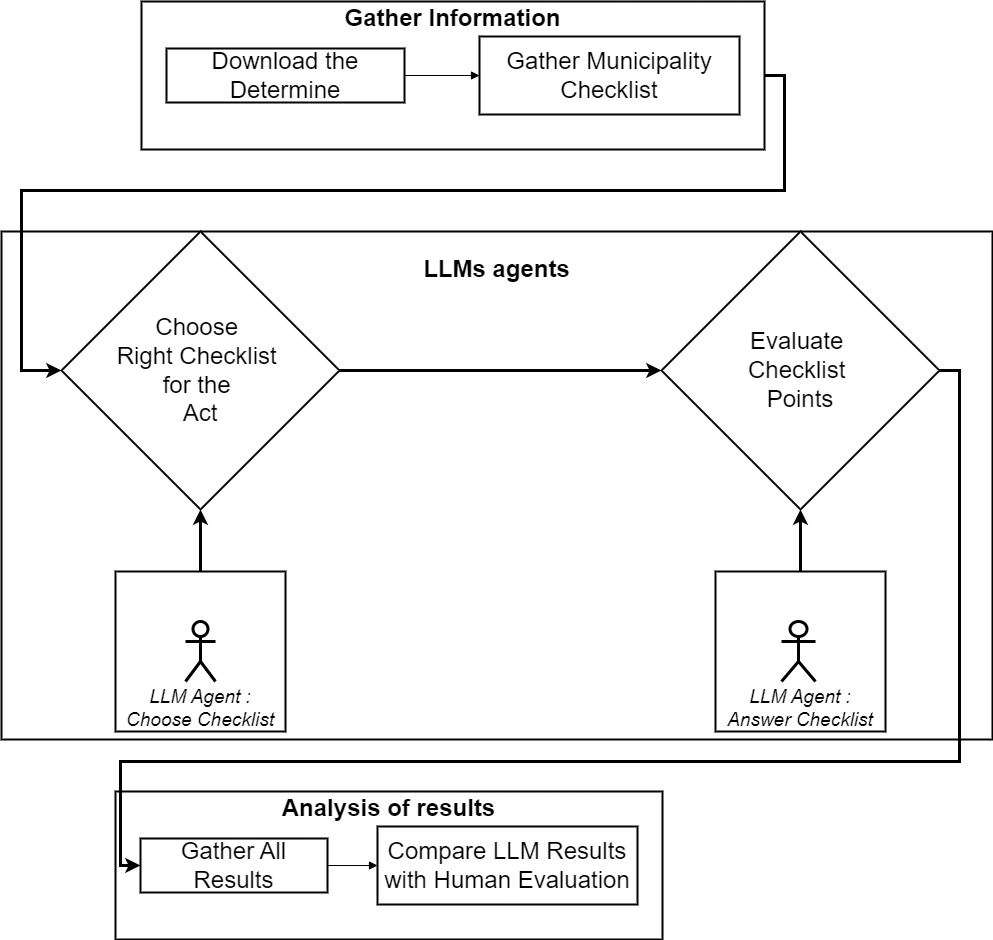
\includegraphics[width=10cm]{0.Workflow.png}
\end{figure}

\section*{Tools and Performance Metrics}
Several tools and performance metrics were used throughout the study:

\begin{itemize}
    \item \textbf{Software Tools:}
    \begin{itemize}
        \item Python for text extraction, prompt generation, and response processing.
        \item Regular expressions for cleaning and standardizing text outputs.
        \item OpenAI's API for accessing the LLM.
        \item Hugginface Transformers Library to load and use locally llama models
        \item CSV and JSON file handling for managing checklists and responses.
    \end{itemize}
    \item \textbf{Performance Metrics:}
    \begin{itemize}
        \item \textbf{Accuracy:} The degree to which the LLM's responses match the human-evaluated answers.
        \item \textbf{Consistency:} Variability in outputs with changes in the model's temperature and other parameters.
        \item \textbf{Efficiency:} Processing time and resource usage for automating the evaluation process.
        \item \textbf{Error Rate:} Frequency and nature of errors encountered during response extraction and analysis.
    \end{itemize}
\end{itemize}

\end{document}